% exercise sheet with header on every page for math or close subjects
\documentclass[12pt]{article}
\usepackage[utf8]{inputenc}
\usepackage{latexsym}
\usepackage{multicol}
\usepackage{fancyhdr}
\usepackage{amsfonts}
\usepackage{amsmath}
\usepackage{amssymb}
\usepackage{enumerate}
\usepackage{listings}
\usepackage{graphicx}

% Shortcuts for bb, frak and cal letters
\newcommand{\E}{\mathbb{E}}
\newcommand{\V}{\mathbb{V}}
\renewcommand{\P}{\mathbb{P}}
\newcommand{\N}{\mathbb{N}}
\newcommand{\R}{\mathbb{R}}
\newcommand{\C}{\mathbb{C}}
\newcommand{\Z}{\mathbb{Z}}
\newcommand{\Pfrak}{\mathfrak{P}}
\newcommand{\Pfrac}{\mathfrak{P}}
\newcommand{\Bfrac}{\mathfrak{P}}
\newcommand{\Bfrak}{\mathfrak{B}}
\newcommand{\Fcal}{\mathcal{F}}
\newcommand{\Ycal}{\mathcal{Y}}
\newcommand{\Bcal}{\mathcal{B}}
\newcommand{\Acal}{\mathcal{A}}

% formating
\topmargin -3.5cm
\textheight 22cm
\textwidth 16.0 cm
\oddsidemargin -0.1cm

% Fancy Header on every Page
\pagestyle{fancy}
\lhead{\textbf{Embedded Systems Problem Set A}}
\rhead{Daniel Schäfer (2549458)\\ Rafael Dewes ()\\ Kevin M\"uller (2550062)}
\renewcommand{\headrulewidth}{1.2pt}
\setlength{\headheight}{110pt}

\begin{document}
\pagenumbering{gobble}
\lstset{language=C++}

\section*{Problem A1}

For an equilibrium the car would not be allowed to move (velocity 0, which means derivative of its position equals zero) and the derivative of its velocity would have to be zero.

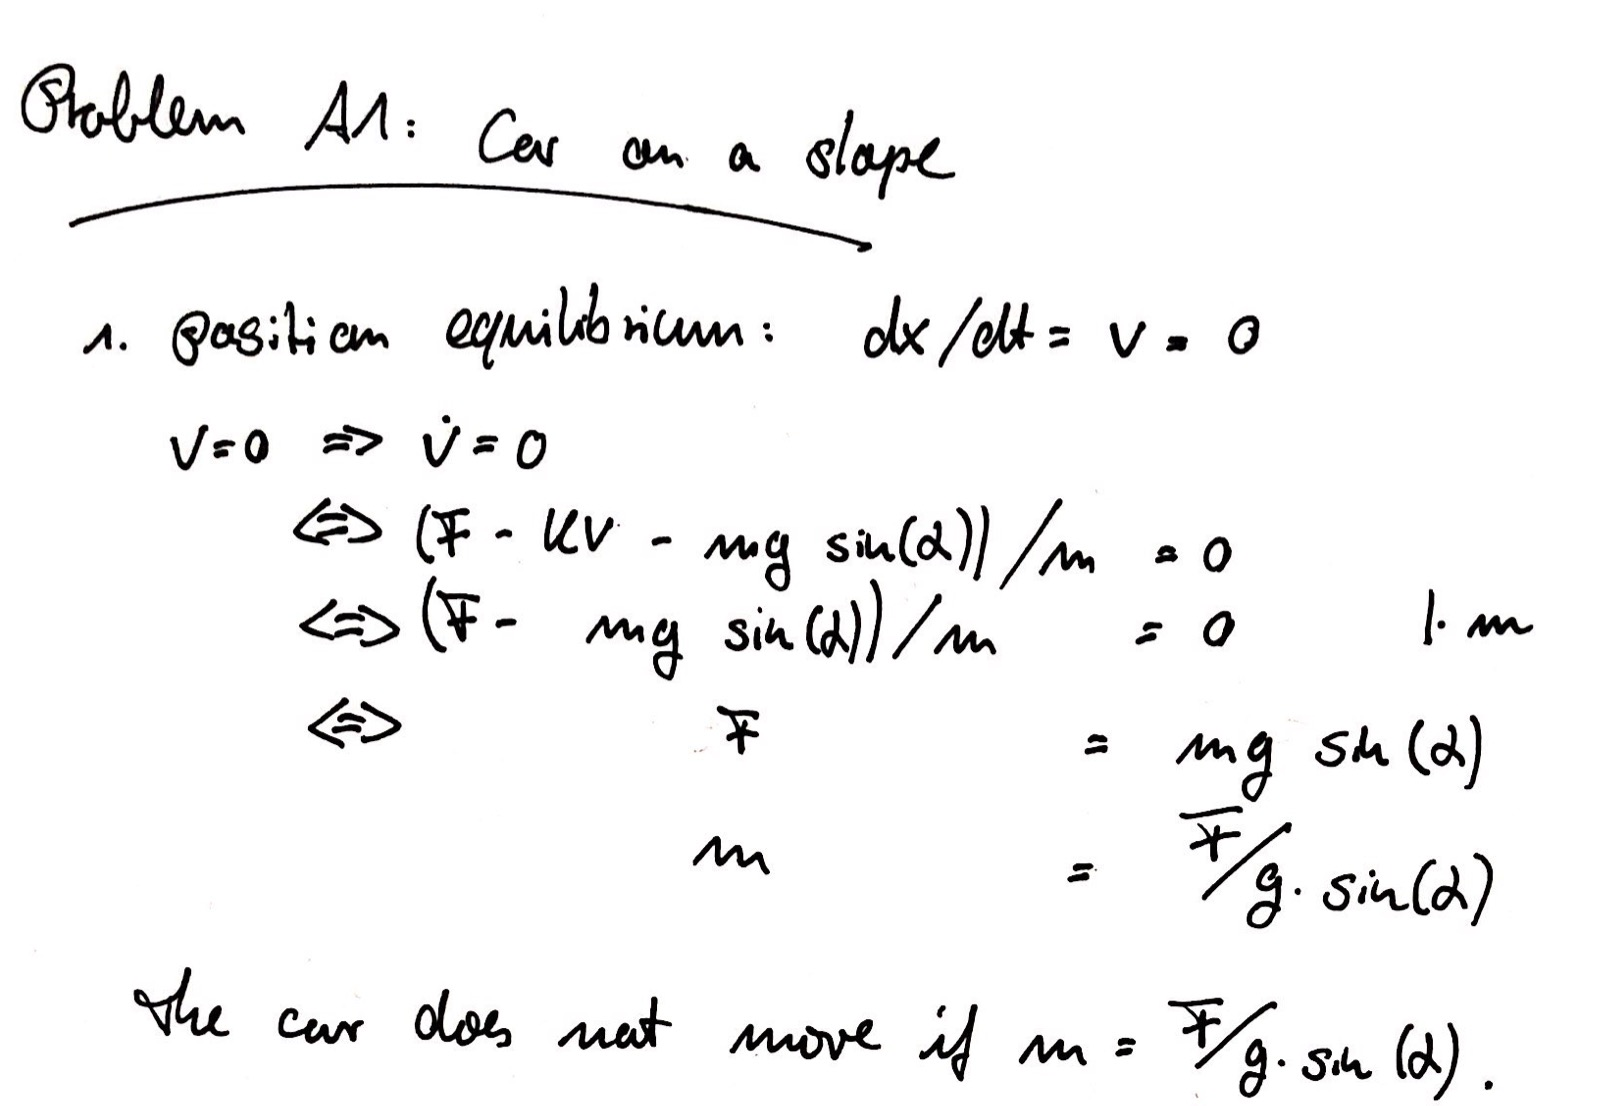
\includegraphics[scale = 0.29]{pictures/pa1}\\

In the case where the car does not accelerate (i.e. $F=0$), it can only reach an equilibrium if $\alpha = 0$


\section*{Problem A2}
\begin{enumerate}[a)]
  \item 
      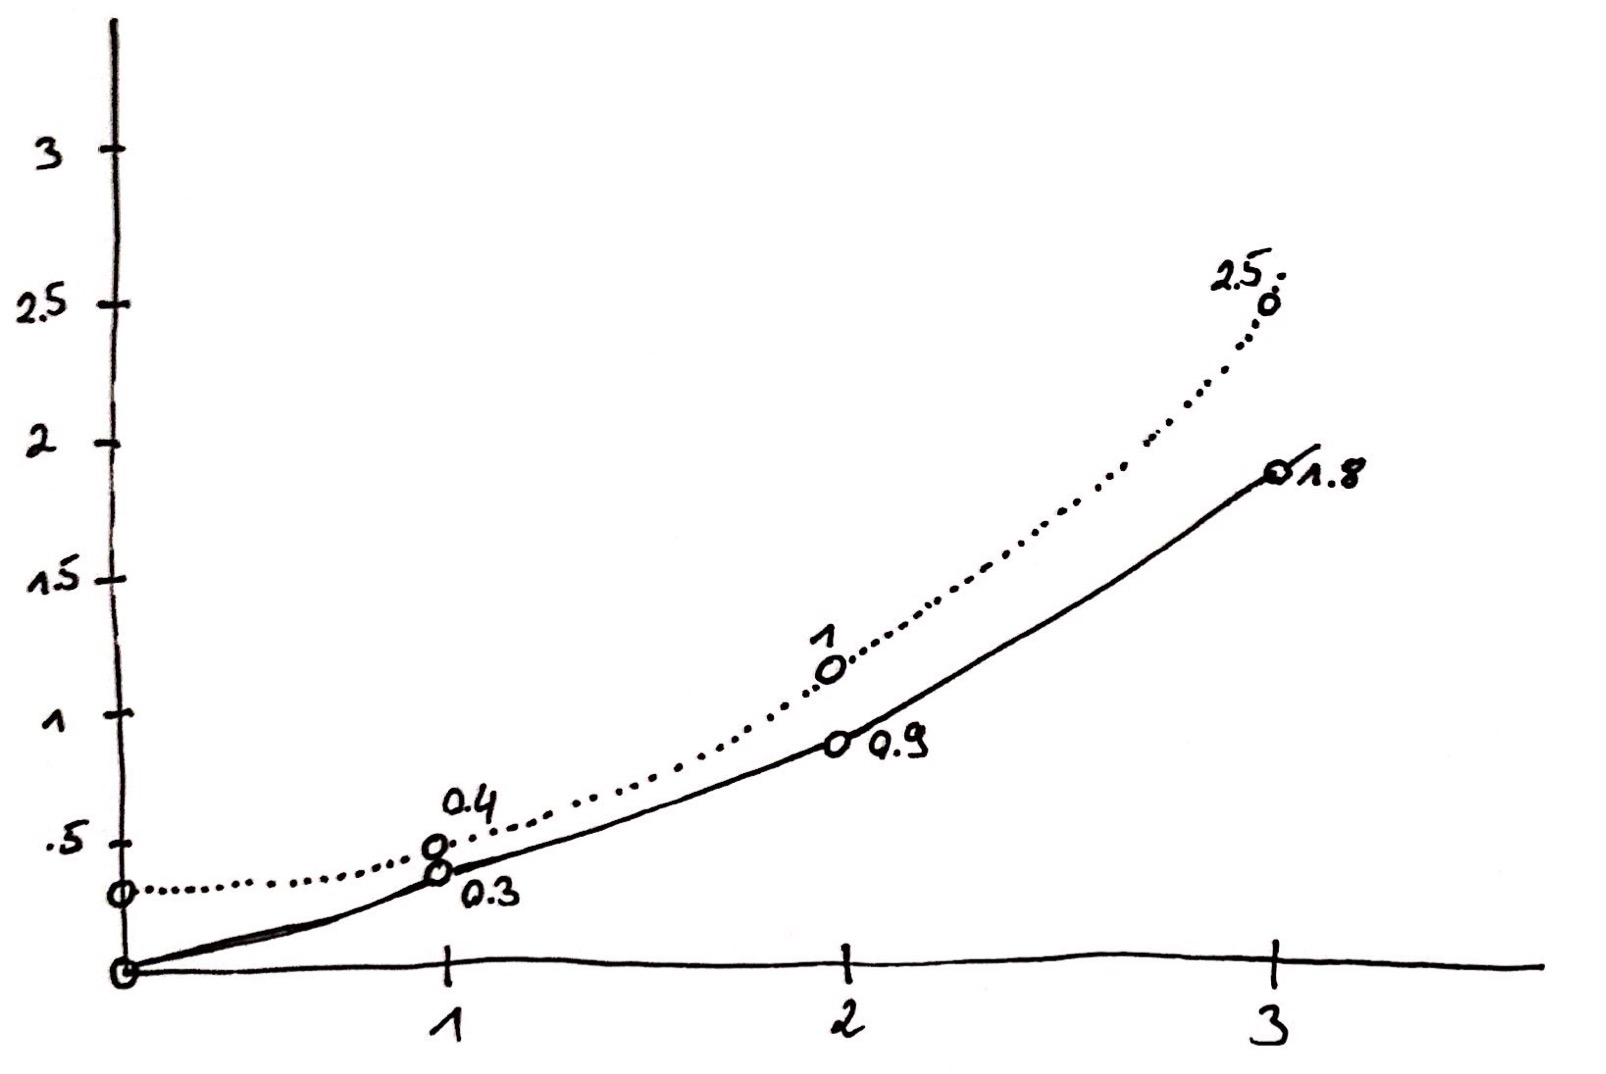
\includegraphics[scale = 0.22]{pictures/pa2a}\\
  \item 
      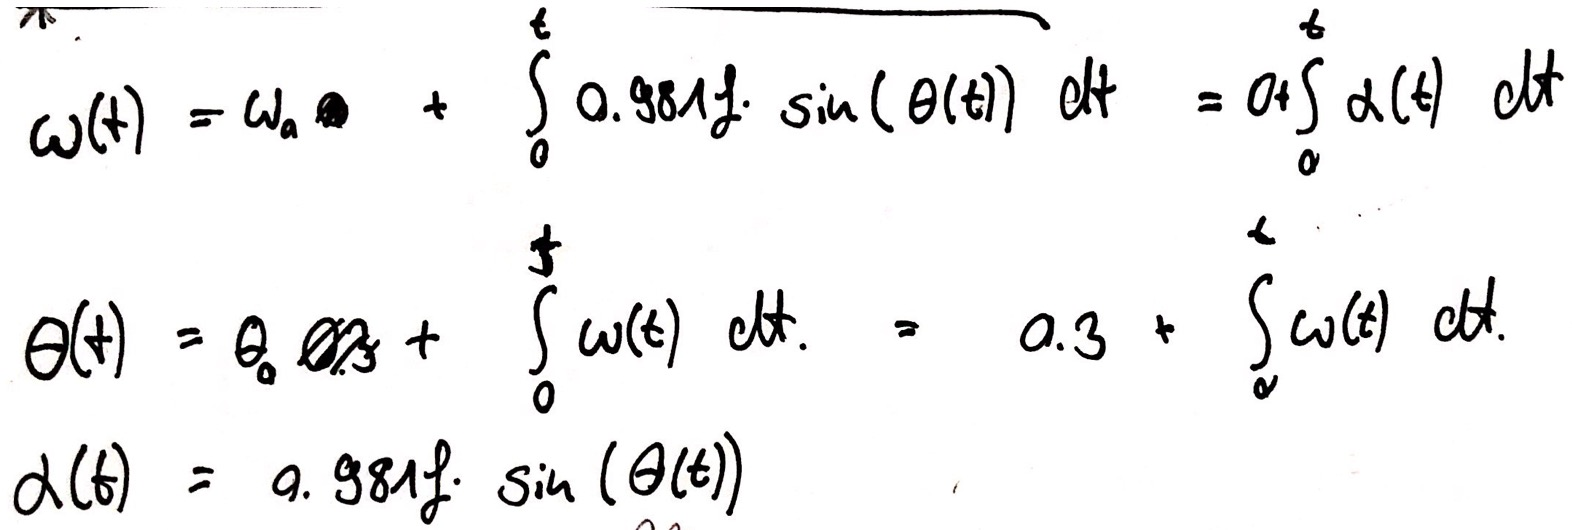
\includegraphics[scale = 0.22]{pictures/pa2b}\\
  \item All outputs are upper bound by some constant because of the following arguments:
  \begin{itemize}
    \item Alpha will always be upper bound by $1* \frac{g}{l} * f$ because sinus moves continiously between $-1$ and $1$ as it is periodic.
    \item this results in the rate of change being limited by an upper bound because f is also bounded according to BIBO stability assumptions.
    \item Essentially alpha (which is upper bound) limits the rate of growth for omega, which makes this upper bound. Analogously theta is limited by the limited rate of change introduced by omega being upper bound.

  \end{itemize}
\end{enumerate}


\section*{Problem A3}
For this function to be Lipschitz continious, the derivative of the function would have to be bounded by some constant.

$$f'(x) = -\frac{1}{2} x^{-\frac{1}{2}} \quad \quad x > 0$$
$$f'(x) = \frac{1}{2} -x^{-\frac{1}{2}} \quad \quad x < 0$$

$$lim_{x \rightarrow 0^-} f'(x) = -\infty$$
$$lim_{x \rightarrow 0^+} f'(x) = +\infty$$

As shown in the limes values above, the derivative of the given function is not bound by some constant, which means that the given function can also not be Lipschitz continious.

\newpage
\section*{Problem A4}

\begin{enumerate}[a)]
  \item 
      See following Diagram:\\
    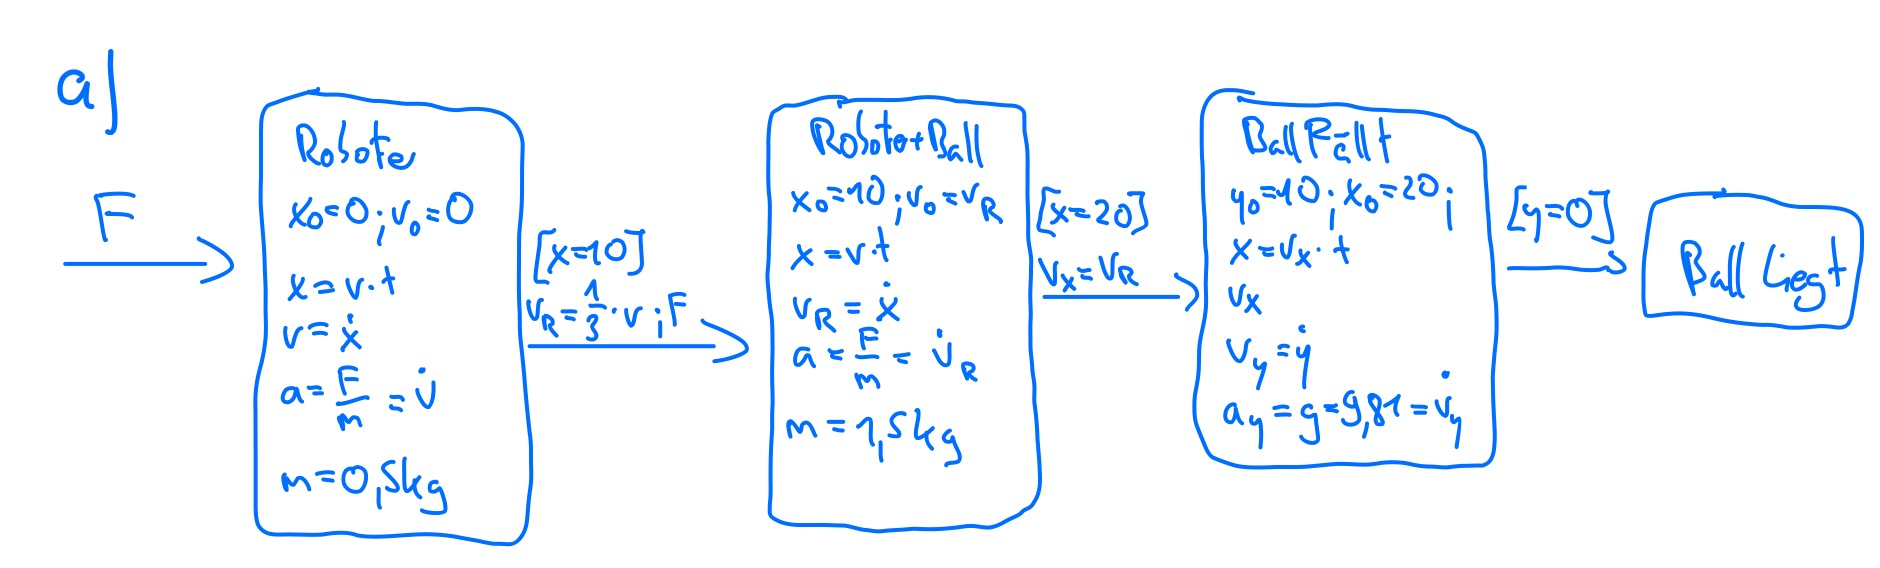
\includegraphics[scale = 0.23]{pictures/pa4a}\\
  \item
      \textbf{Model Overview:}\\
    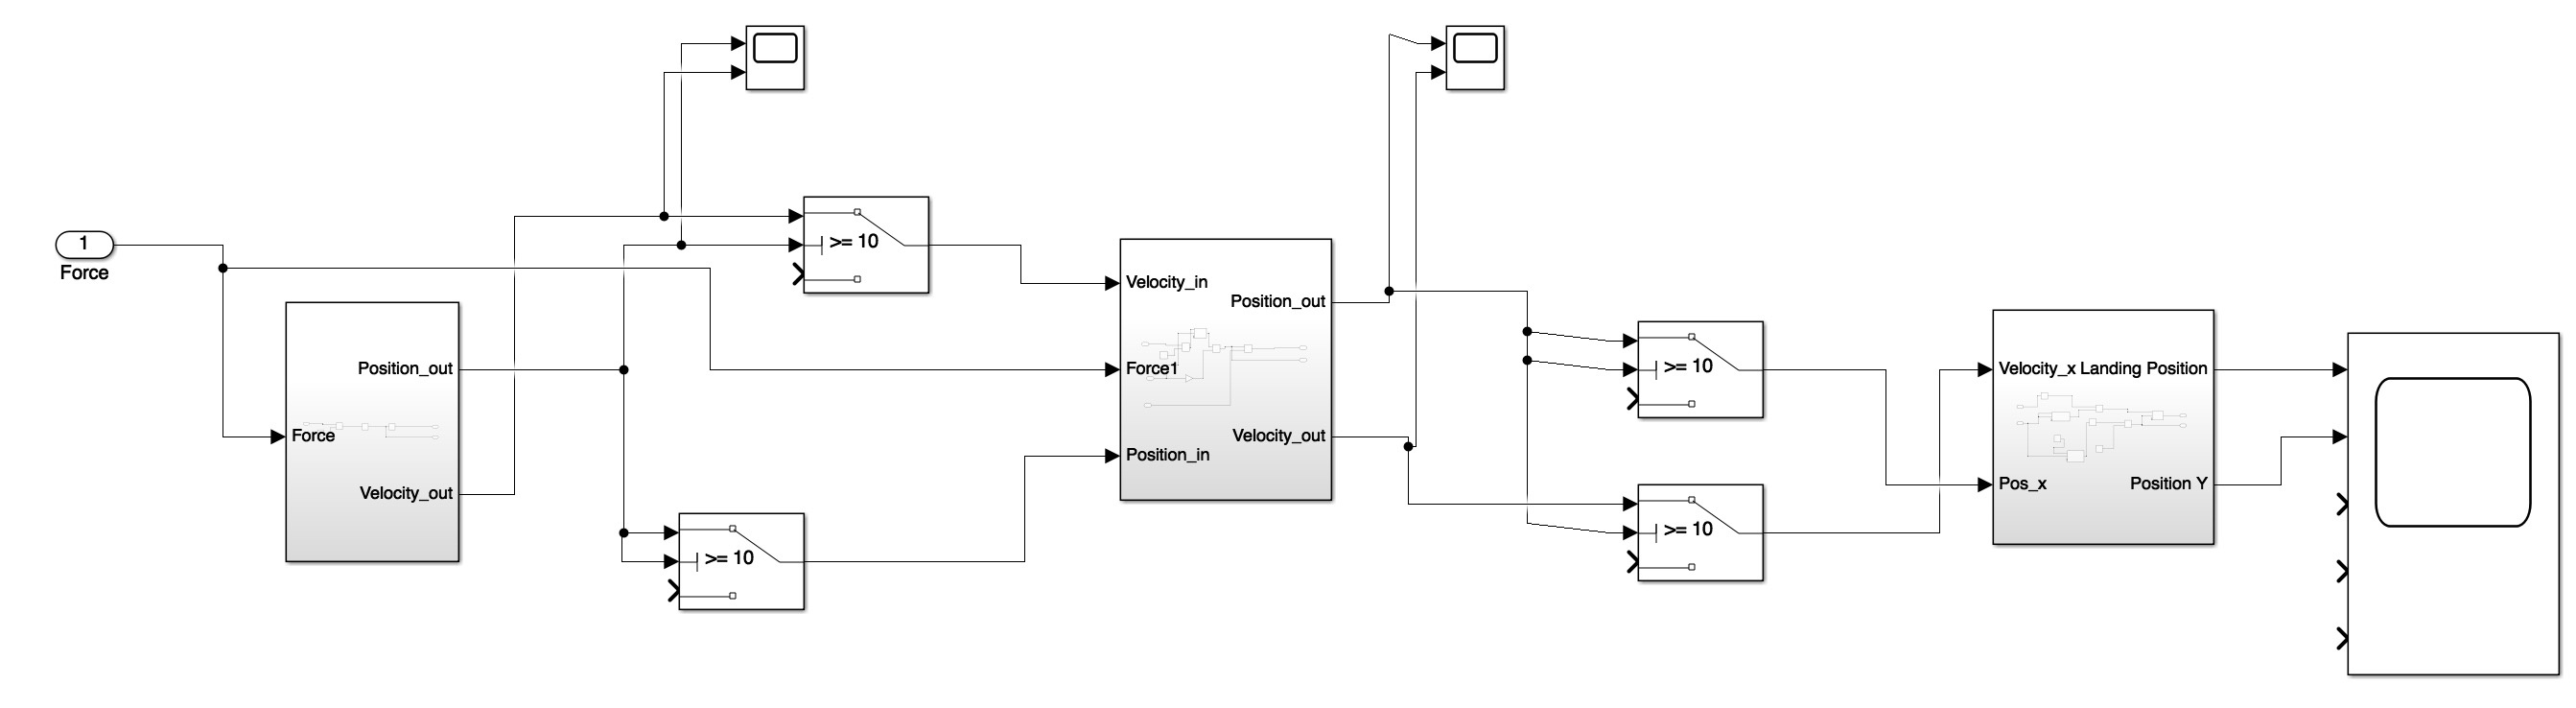
\includegraphics[scale = 0.19]{pictures/model1}\\
    Subsystem Roboter Driving:\\
    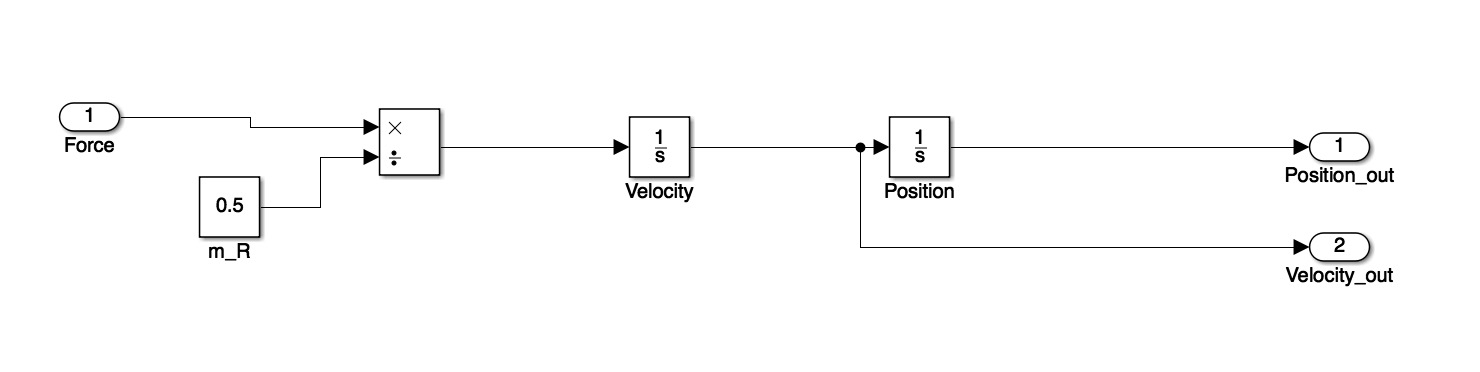
\includegraphics[scale = 0.29]{pictures/model2}\\
    \newpage
      Subsystem Roboter Pushing Ball:\\
    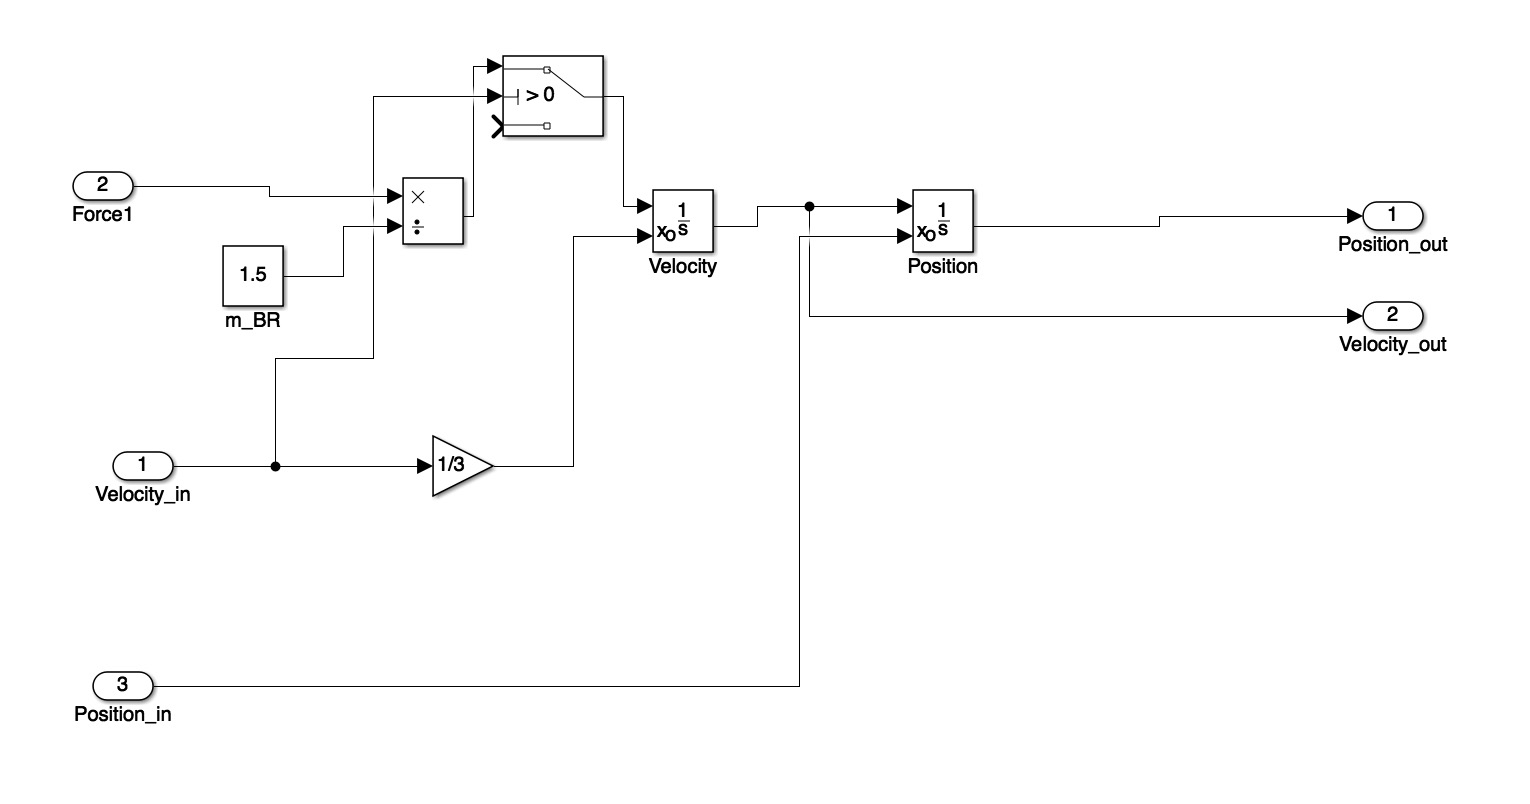
\includegraphics[scale = 0.29]{pictures/model3}\\
      Subsystem Ball Falling over Edge:\\
    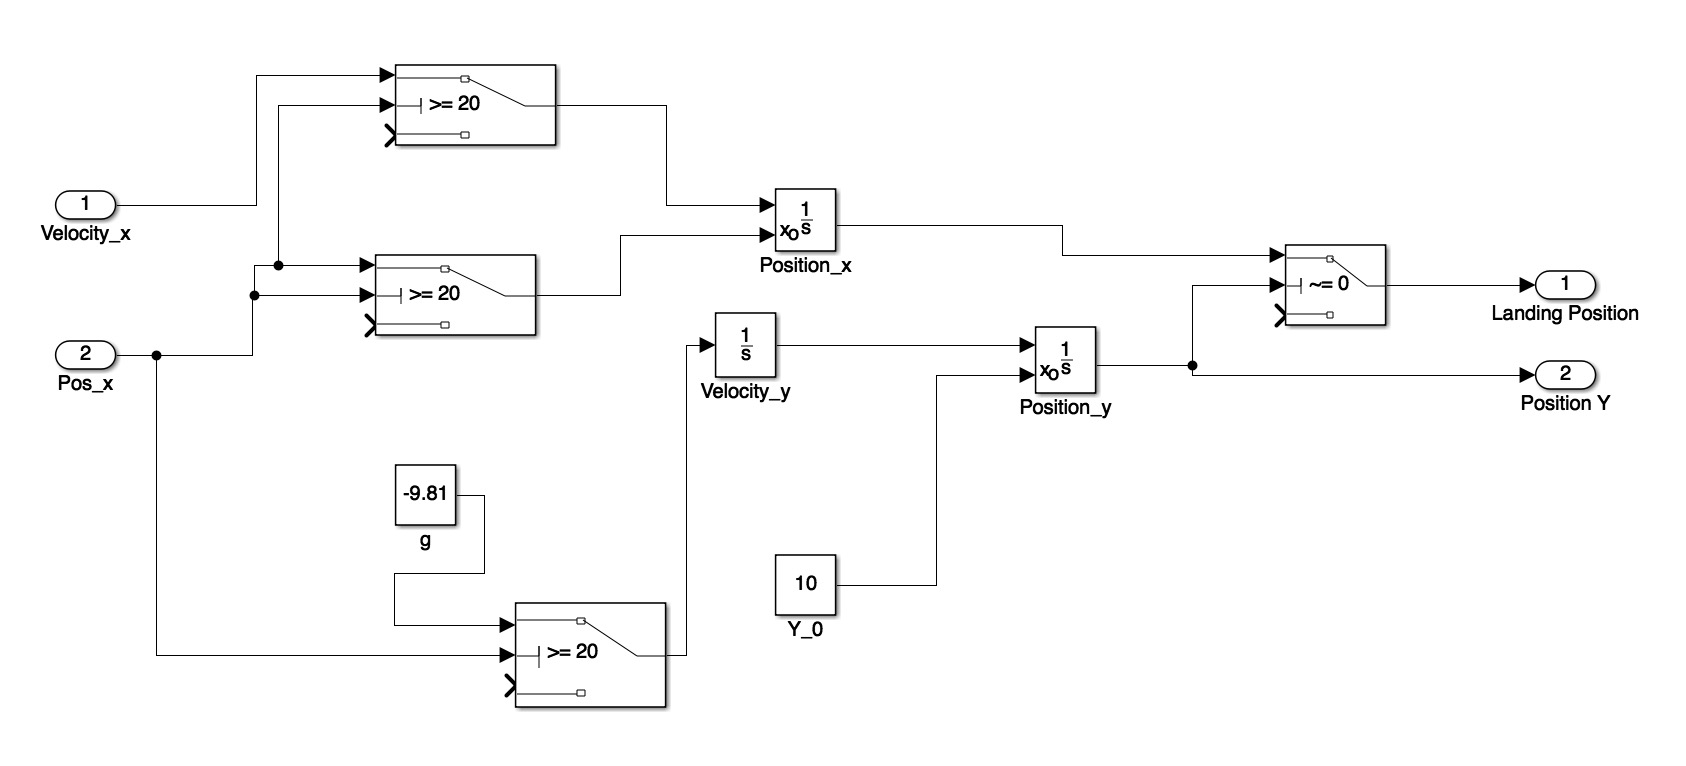
\includegraphics[scale = 0.29]{pictures/model4}\\
    \newpage
      Resulting Plot (only falling phase for N=5):\\
    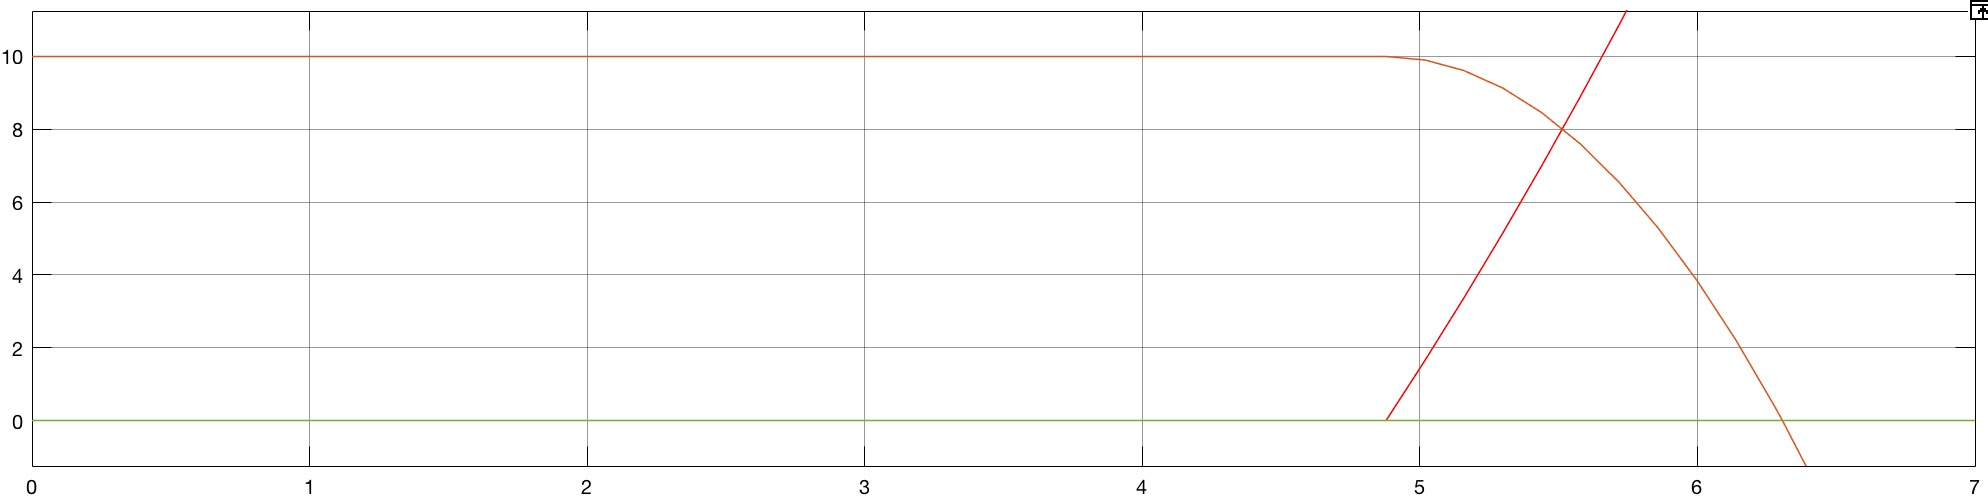
\includegraphics[scale = 0.20]{pictures/falling_5}\\
\newpage
  \item 
    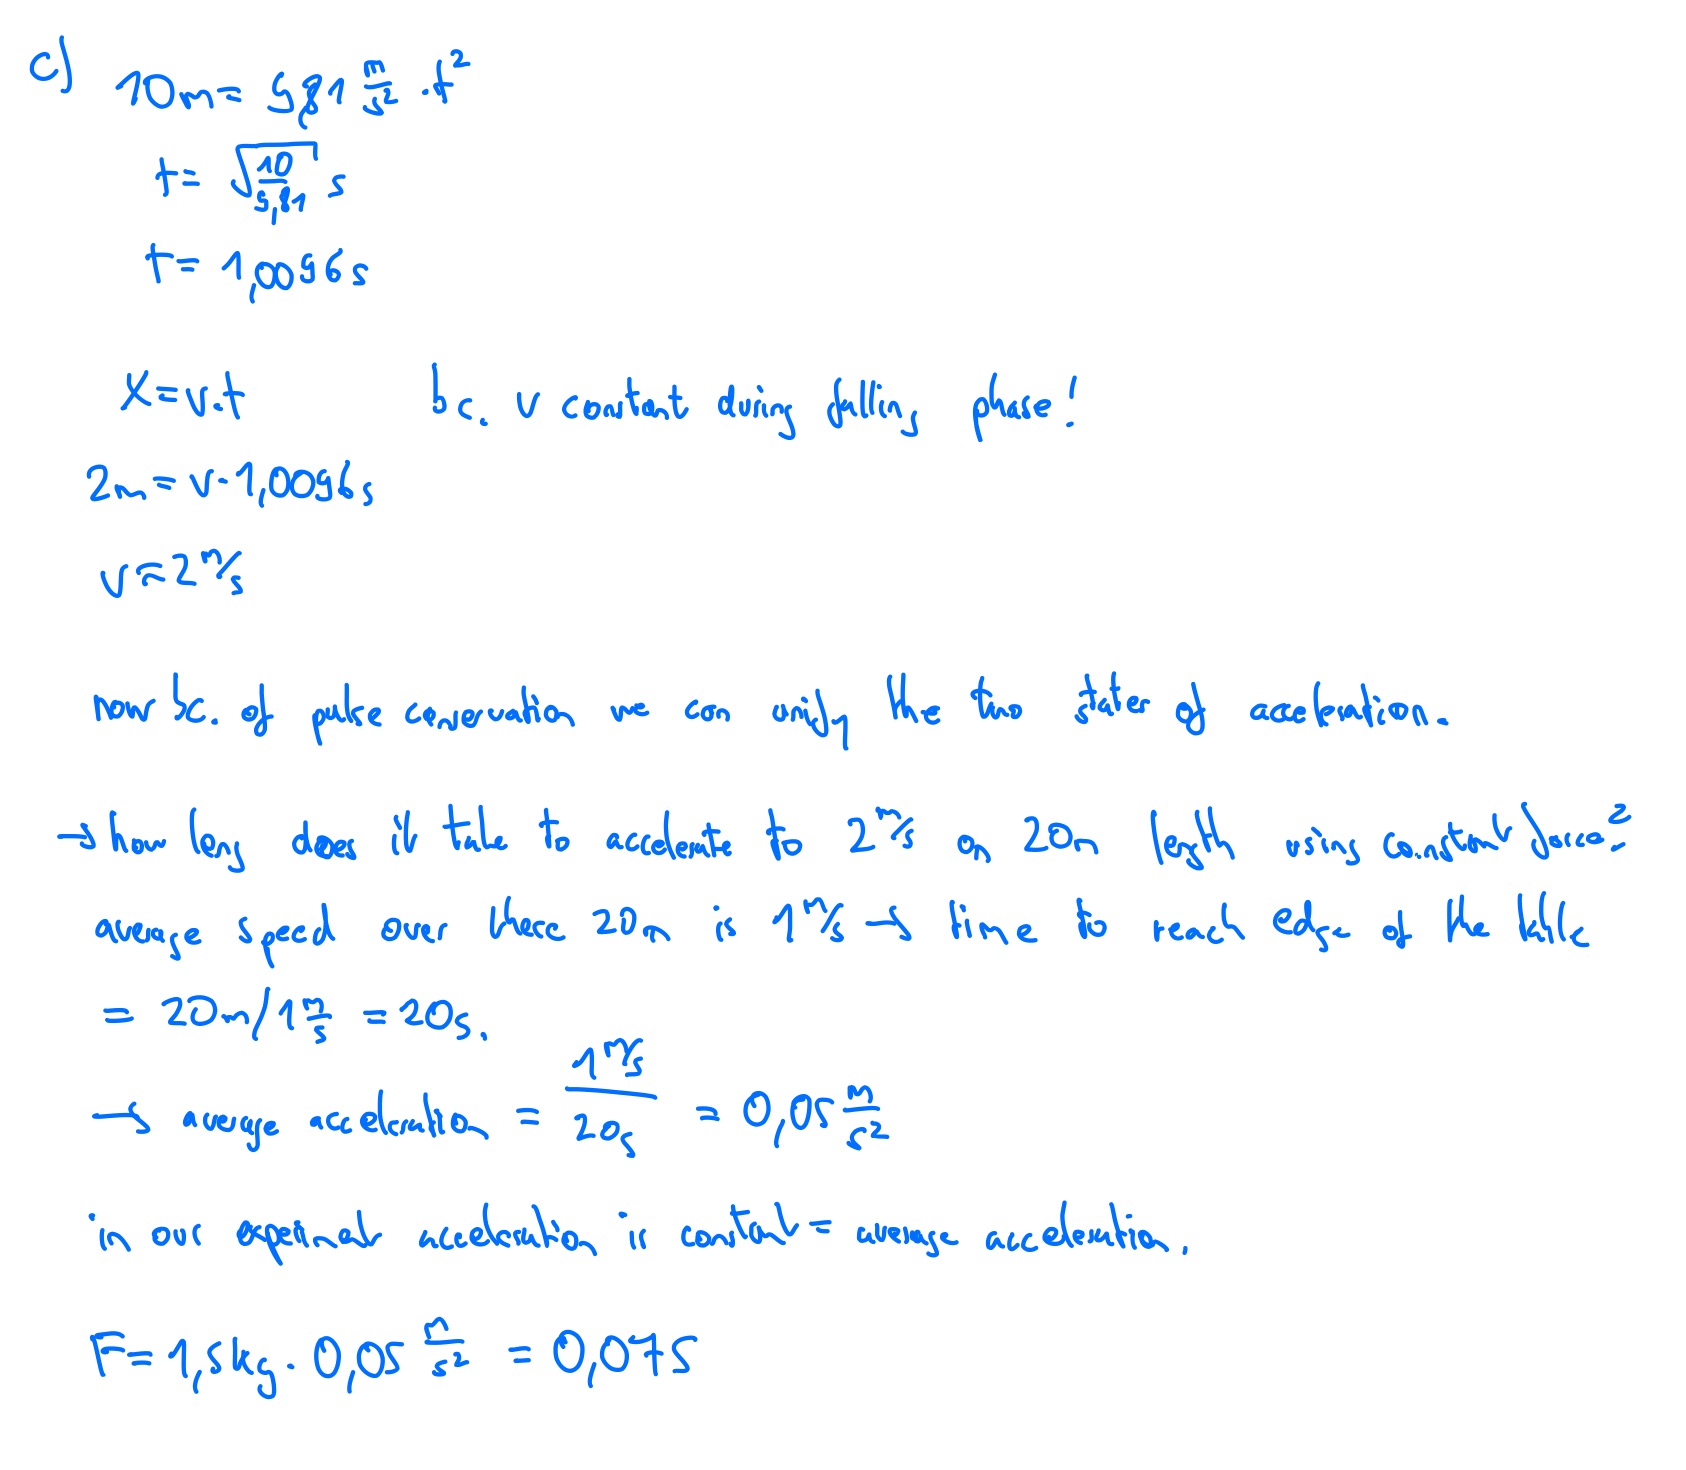
\includegraphics[scale = 0.26]{pictures/pa4c}\\
    We verified this result in our Simulink implementation as shown in the plot below (Plot only contains Falling phase):\\
    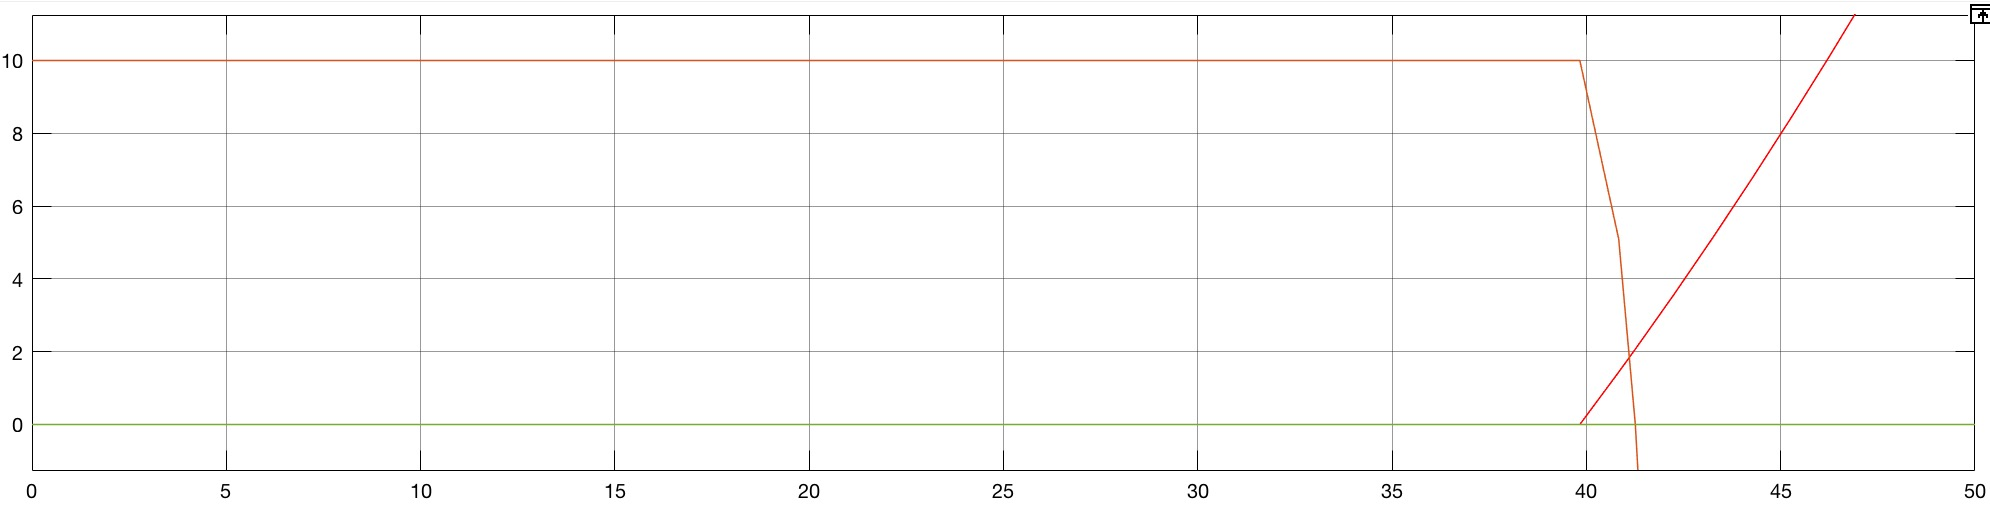
\includegraphics[scale = 0.20]{pictures/falling_0075}\\
\end{enumerate}


\end{document}
